\documentclass[conference]{IEEEtran}
% Draft, 2026-11-24. Simulation only. Numbers come from the result files named in docs/note/analysis_note_draft.md.
\usepackage{graphicx}
\usepackage{booktabs}
\usepackage{amsmath,amssymb}
\usepackage{xcolor}
\usepackage[hidelinks]{hyperref}
\usepackage{cite}
\newcommand{\figdir}{../report/figs}
\newcommand{\pending}[1]{\textcolor{orange}{[pending: #1]}}

\title{Shadows Bias Feature-Field Object Trackers\\Through an Implicit Silhouette Term}
\author{\IEEEauthorblockN{[Author names]}\IEEEauthorblockA{[Affiliation]}}

\begin{document}
\maketitle

\begin{abstract}
Trackers that optimise the pose of a Gaussian splat with distilled DINO features against live image features
report high recovery rates for tools under perturbation. We re-implement one such tracker, POGS, in simulation
with exact ground truth. The published recovery rule leaves roll about the tool axis free, and it hides a
systematic roll error of $9.5 \pm 2.8^\circ$ that is present before any perturbation; under a full rotation rule
recovery falls from 17--39 to 2--14 of 50 trials. The error is not an optimisation failure: the loss prefers the
wrong pose on 87--100\% of frames. Its source is the part of the region-of-interest feature loss that compares
background pixels with an empty render, an implicit silhouette term. On three independently trained splats the
roll minimum follows the strength of the gripper's cast shadow (Spearman $\rho \leq -0.85$, shifts of 5--9$^\circ$),
while the same loss with a rendered background moves by at most $1.5^\circ$; the loss of RSRD, the tracker POGS
derives from, shows the same bias. Pre-registered tests also refute our initial hypothesis that this term supplies
the restoring force: the object's own features provide most of the local stiffness in rotation and translation.
Six corrections fail a criterion fixed in advance. We give evaluation rules, with code: report both rules, score a
no-motion baseline, and decompose roll from swing.
\end{abstract}

\section{Introduction}
Persistent feature fields let a robot track an object it has scanned once: a Gaussian splat~\cite{kerbl2023gaussian}
is distilled with DINO features~\cite{oquab2024dinov2}, and at run time the object pose is found by rendering
those features and matching them to the live image~\cite{kerr2024rsrd,yu2025pogs}. POGS~\cite{yu2025pogs} reports
48 of 50 drill recoveries for perturbations up to $15^\circ$ and 40 of 50 at $30^\circ$.

We set out to reproduce this result and to understand what limits it. Our contributions:
\begin{enumerate}
\item \textbf{An evaluation finding.} The published rule is roll-free. Under it our re-implementation matches the
paper's $30^\circ$ tier in one direction ($39$ vs.\ $40$ of 50, Fisher $p=1.0$); under a full rotation rule recovery
collapses, and a relative ``back to pre-perturbation error'' rule is passed by a tracker that does not move.
\item \textbf{A bias mechanism, replicated.} The ROI-averaged feature loss contains an implicit silhouette term
(background vs.\ an empty render) that carries a shadow- and viewpoint-dependent bias, with a dose-response on three
splats and in a second objective, RSRD's (Sec.~\ref{sec:mechanism}, \ref{sec:g1}). This links feature-field trackers to region-based silhouette trackers, for which
sensitivity to shadows and background is well known~\cite{prisacariu2012pwp3d,stoiber2022srt3d}.
\item \textbf{Negative results with fixed criteria}: the term does not supply the static restoring force
(three pre-registered tests), and six corrections fail (Sec.~\ref{sec:fixes}).
\item \textbf{Evaluation rules} with code (Sec.~\ref{sec:recs}).
\end{enumerate}

\section{Related work}
\textbf{Feature-field tracking.} RSRD~\cite{kerr2024rsrd} recovers part motion from monocular video by optimising
part poses of a DINO-embedded splat; POGS~\cite{yu2025pogs} adds grouping and persistent tracking with depth.
Both average a feature loss over the ROI, with the object-only render as the prediction (Sec.~\ref{sec:g2}).
Analysis-by-synthesis pose estimation with radiance fields started with iNeRF~\cite{yen2021inerf}; Gaussian-splat
trackers with RGB or mask objectives include 6DOPE-GS~\cite{jin20246dope} and GSGTrack~\cite{gsgtrack2024}.
\textbf{Region-based tracking.} PWP3D~\cite{prisacariu2012pwp3d} and SRT3D~\cite{stoiber2022srt3d} optimise a pose
so that the projected silhouette separates foreground and background statistics; we show that a feature-field
loss contains such a term implicitly, and that it, not the object features, carries the shadow bias. \textbf{Evaluation.} Pose metrics that are ambiguous under symmetries or
free DOF are discussed in~\cite{hodan2016evaluation}; we add the case of a rule that frees a DOF in which the
tracker is biased.

\section{Setup}
Re-implementation of the POGS release (DINOv2 ViT-S/14, PCA-64, ROI DINO L2 + depth, Adam, 25 iterations per frame)
in a simulator with exact ground truth. Tool scene: a procedural drill on a table among five household objects,
35-view capture, one splat (PSNR 33.5). In-grasp perturbation protocol after the paper: grasp, lift, rotate by
$\pm15^\circ$ or $\pm30^\circ$, return; 50 seeds per setting. Every table includes Static (the pose never updated).

\section{The recovery rule hides a roll bias}
\begin{table}[t]\centering\caption{Recovery out of 50 by rule. Paper: 48 (Tier 1), 40 (Tier 2).}\label{tab:rules}
\begin{tabular}{lccc}\toprule
Setting & Full rule & Roll-free (paper) & Static \\\midrule
$+15^\circ$ & 2 & 32 & 0\\ $-15^\circ$ & 14 & 25 & 0\\ $+30^\circ$ & 13 & 39 & 0\\ $-30^\circ$ & 5 & 17 & 0\\\bottomrule
\end{tabular}\end{table}
94\% of the pre-perturbation rotation error is roll about the bit axis ($|\text{roll}| = 9.5\pm2.8^\circ$, swing
$4.0\pm3.4^\circ$). The error is already $12.5^\circ$ at the end of the approach, before the gripper touches the drill.
Its sign is positive in 167 of 200 trials, which explains why $+$ perturbations recover more often than $-$
(Fig.~\ref{fig:roll}). A filter does not change it.
\begin{figure}[t]\centering\includegraphics[width=\linewidth]{\figdir/o4_roll_trace.pdf}
\caption{Median roll about the bit axis and swing of the axis over the in-grasp trials (200 trials).}\label{fig:roll}\end{figure}

\section{Mechanism: a biased implicit silhouette term}\label{sec:mechanism}
Let $e(p)=\lVert f(p)-\hat f_\theta(p)\rVert$ be the per-pixel feature residual in an ROI of $N$ pixels, with
$\hat f_\theta$ the blurred object-only render at pose $\theta$. With $M(\theta)$ the rendered object mask,
\begin{align}
L(\theta)&=\tfrac1N\textstyle\sum_{p} e(p)=S_\text{in}(\theta)+S_\text{out}(\theta),\\
S_\text{in}&=\tfrac1N\textstyle\sum_{p\in M(\theta)} e(p),\nonumber\\
S_\text{out}&=\tfrac1N\textstyle\sum_{p\notin M(\theta)} e(p)\approx\tfrac1N\textstyle\sum_{p\notin M(\theta)}\lVert f(p)\rVert .\nonumber
\end{align}
Off the object the render is close to zero, so $S_\text{out}$ is the summed norm of the live features that the predicted
silhouette leaves uncovered: a silhouette term. In the drill ROI 87\% of pixels are background.
\textbf{Evidence.} (i) The ground truth is exact: RGB-only argmins are at $0.0^\circ$ in every rotation. (ii) The
features inside the drill are unbiased: restricted to the true-pose mask, the DINO minimum is within $1^\circ$ of
the truth in all 16 views. (iii) The full-ROI minimum sits at $-10^\circ$ at the tracking camera with the gripper's
shadow, $-6^\circ$ without the gripper and $-2^\circ$ with shadows off. (iv) Removing the background breaks tracking in
trajectories: DINO inside the per-pose mask tracks 1/0/4/4 of 25 vs.\ 9/12/16/23 for POGS; switching DINO off
(depth only) gives 0 everywhere. Static sweeps do not show the background supplying the local rotational
stiffness (Sec.~\ref{sec:g1}); the masked variants fail through translation drift in the lift.
\textbf{Dose-response.} Scaling the cast-shadow strength $s$ of the tracking frame (gripper at its frame-0 pose)
moves the roll minimum monotonically on all three independently trained splats (Fig.~\ref{fig:dose}; Spearman
$\rho=-0.97,-0.85,-0.85$; shift from $s=0$ to $s=1$ of $-8.0^\circ$, $-9.0^\circ$, $-5.0^\circ$). The same loss with a
rendered background moves by $0.5$--$1.5^\circ$ and stays at $+2$ to $+4^\circ$. Both pre-registered rules (P4, P5) pass.
\begin{figure}[t]\centering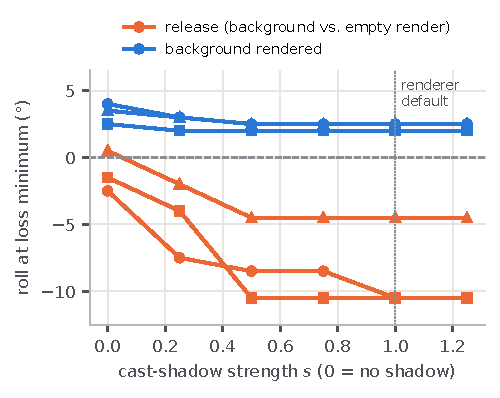
\includegraphics[width=\linewidth]{figs/dose_response.pdf}
\caption{Dose-response: roll at the minimum of the DINO loss vs.\ cast-shadow strength, drill at the true pose,
three splats (markers). Only the tracking frame is re-rendered; the splats were trained at $s=1$.}\label{fig:dose}
\end{figure}
\begin{figure}[t]\centering\includegraphics[width=\linewidth]{\figdir/finding_argmin.pdf}
\caption{Roll argmin of each loss term at the true pose.}\label{fig:argmin}\end{figure}

\section{Generality}\label{sec:g1}
We pre-registered five predictions (\nolinkurl{docs/note/g1_generality_preregistration.md}) before any sweep: three
splats of the tool scene trained with different seeds; four objects (drill, mug, mustard bottle, cereal box);
the tracking camera with and without shadows and 12 held-out views; rotations about three axes. Results, in the
order fixed in advance:
\begin{table}[t]\centering\caption{Pre-registered generality results (static sweeps).}\label{tab:g1}
\small\begin{tabular}{@{}p{0.6\linewidth}p{0.33\linewidth}@{}}\toprule Prediction & Result\\\midrule
P1: background carries $>50\%$ of the local rotational curvature ($\geq3$/4 objects; drill on new splats) & fail (2/4; drill 0.10, 0.17, 0.27)\\
P2: drill roll bias $\leq-5^\circ$ replicates on new splats & pass ($-10, -10, -5^\circ$)\\
P3: rendered background lowers mean $|$argmin$|$ on held-out views ($\geq3$/4) & fail (2/4)\\
P4: monotone shadow dose-response ($\geq2$/3 splats) & pass (3/3)\\
P5: rendered background moves $<$ half as much ($\geq2$/3) & pass (3/3)\\\bottomrule
\end{tabular}\end{table}
The bias and its dependence on shadow replicate across splats (P2, P4, P5). The stronger claim we started with, that
the background term supplies most of the restoring force, does not hold for rotation: near the truth the object's
own features give most of the curvature (P1), and the rotational basins are about $\pm20^\circ$ wide with or without
the background term. A caveat on P1: the split $S_\text{in}+S_\text{out}$ uses the mask at the evaluated pose, so
pixels crossing the silhouette are counted inside; it is not a clean causal split. Because the masked variants failed in trajectories through translation drift, we pre-registered one more test
after reading P1 (\nolinkurl{docs/note/g1b_translation_preregistration.md}): the object features supply less than
half of the translational stiffness for at least 3 of 4 objects. It fails (0/4): their share is 0.75--1.00, and a
rendered background gives 1.4--1.6 times the release stiffness. Static sweeps therefore do not explain why tracking
without the background term fails; that failure is dynamic (gripper occlusion, mask feedback), and we leave it open.
\subsection{A second tracker: the RSRD objective}\label{sec:g2}
RSRD~\cite{kerr2024rsrd} builds its DINO loss the same way (object-only render, sharp inside the mask and blurred
outside, averaged over the ROI) and adds an RGB L1 term over the ROI, also against the object-only render.
We evaluated RSRD's objective (DINO term as above, $+0.05\times$ RGB L1, metric depth inside the mask) with our splat
and renderer, pre-registered (\nolinkurl{docs/note/g2_second_tracker_preregistration.md}). As for POGS, the background
does not carry most of the curvature (Q1, Q2: 0/4 objects; drill 0.09), but the drill's roll minimum with the
gripper's shadow is at $-10^\circ$ (Q3, pass), the same as POGS. RSRD and POGS share code lineage, so this tests the objective family, not an
independent implementation.

\section{Corrections tested}\label{sec:fixes}
Pass rule fixed before the runs: paired roll-free bootstrap CI above zero in at least 2 of 4 settings and below zero
in none, lower pre-perturbation roll, and better than a depth-only control in at least 2 settings.
\begin{table}[t]\centering\caption{Corrections, roll-free recoveries out of 25 ($-30/-15/+15/+30^\circ$).}\label{tab:fixes}
\begin{tabular}{lcc}\toprule Variant & Recoveries & Pass\\\midrule
POGS (release) & 9/12/16/23 & ref.\\
RGB term, weight 1 & 16/13/20/18 & no\\
Depth $\times30$ & 2/1/0/0 & no\\ Depth $\times100$ & 0/0/0/0 & no\\
DINO inside object mask & 1/0/4/4 & no\\ DINO vs.\ rendered background & 0/0/0/0 & no\\
Depth only (DINO off) & 0/0/0/0 & control\\\bottomrule\end{tabular}\end{table}
Re-distilled features (DINOv2 with registers, DINOv3 ViT-S/16, AnyUp upsampling) fail on held-out views before
any trajectory is run. The rendered background removes the bias on static frames (frame 2: $0.6^\circ$ vs.\ $15.1^\circ$)
but the static scene is stale once the drill moves.

\section{Recommendations for tool-tracking evaluation}\label{sec:recs}
(1) Report the full and the tool-axis rule side by side and say which DOF a rule frees. (2) Score every rule on a
no-motion baseline; do not use relative rules, or stratify them by the sign of the pre-existing error. (3) Store
full SE(3) per frame and decompose error into roll and swing. (4) Sweep the loss at the true pose, term by term,
across views and lighting, before attributing an error to observability. A reference implementation
(\texttt{metrics/recovery\_report.py}) produces all of these in one call.

\section{Limitations}
Simulation, one procedural drill, one lighting model; real cameras add exposure changes. The paired $\pm$
asymmetry is not explained by the mechanism alone. A shadow-free explicit silhouette (depth foreground with
gripper exclusion) is pre-registered but not run.

\bibliographystyle{IEEEtran}
\bibliography{refs}
\end{document}
